\chapter{Least-Square Approximation}
\label{chap:leastsq}

As discussed in Chapter \ref{chap:SolLinSys}, given a linear system, if the number of equations (rows) is greater than the number of unknowns (columns), then it is overdetermined. Generally, it would be inconsistent and there will be no solution. However, we can salvage this by finding an approximated solution such that the so-called squared error is minimized. This is known as the \textit{least-square approximation}. Its most common application is \textit{linear regression} in which we predict a dependent variable using an optimized linear equation in some independent variable(s).

\section{Mathematical Ideas of Least-Square Approximation}

For a linear system $A\vec{x} = \vec{h}$ where $\vec{h}$ does not lie in $\mathcal{C}(A)$ the column space of $A$, by Properties \ref{proper:consistentcolspace} it is inconsistent and there will be no exact solution. Nevertheless, a best-fit vector $\vec{x}_f$ can be found, where $A\vec{x}_f = \vec{h}_f$, in the sense that $\vec{h}_f$ will be the closest vector in the column space of $A$ to $\vec{h}$ in distance, i.e.\ the squared error
\begin{align*}
\norm{\vec{h}-\vec{h}_f}^2 = \norm{\vec{h}-A\vec{x}_f}^2    
\end{align*}
is minimized and $\vec{h}_f = A\vec{x}_f$ (or $\vec{x}_f$) is referred to as the \index{Least-square Approximation}\keywordhl{least-square approximation} to the system. From Properties \ref{proper:shortestorthoproj}, we know that the shortest distance will be achieved by the orthogonal projection of $\vec{x}$ onto the column space of $A$. Notice that the distance and orthogonality can now be defined with respect to a general inner product other than the usual dot product. Therefore, $\vec{h}-A\vec{x}_f$ will be in the orthogonal complement $\mathcal{C}(A)^\perp$\footnote{which may not be equal to $\mathcal{N}(A^T)$ or $\mathcal{N}(A^*)$ but rather $\mathcal{N}(A^\dag)$ if an inner product other than the standard one is used.} of the column space $\mathcal{C}(A)$ of $A$, and we have
\begin{align*}
\langle A\vec{x}, \vec{h}-A\vec{x}_f \rangle = \langle \vec{x}, A^\dag(\vec{h}-A\vec{x}_f) \rangle = 0 
\end{align*}
Since this holds for any $\vec{x}$, by the last item of Properties \ref{proper:innerprod2} we have
\begin{align*}
A^\dag(\vec{h}-A\vec{x}_f) &= \textbf{0} \\
A^\dag A\vec{x}_f &= A^\dag \vec{h}
\end{align*}
This is called the \index{Normal Equation}\keywordhl{normal equation} due to the appearance of $A^\dag A$. So any $\vec{x}_f$\footnote{The existence of at least one of such a vector is guaranteed by the uniqueness of orthogonal projection of $\vec{h}$ onto $\mathcal{C}(A)$.} satisfying this equation will produce the least-square error. We may be tempted to multiply both sides of the equation by the inverse $(A^\dag A)^{-1}$ to arrive at a formula for the least-square solution $\vec{x}_f = (A^\dag A)^{-1}A^\dag \vec{h}$. However, this is only allowed when this inverse indeed exists, and we now discuss under what condition it will happen.\par
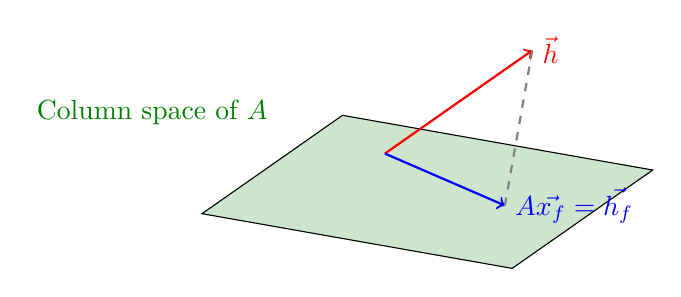
\begin{tikzpicture}[rotate=-10]
\filldraw[fill=Green!20]
(0,0,0) -- (4,0,0) -- (4,0,4) -- (0,0,4) -- cycle;
\draw[red, thick, ->] (1,0,1) -- (3,2,2) node[right]{$\vec{h}$};
\draw[blue, thick, ->] (1,0,1) -- (3,0,2) node[right]{$A\vec{x_f} = \vec{h_f}$};
\draw[gray, thick, dashed] (3,2,2) -- (3,0,2);
\node[Green] at (-2,0,1) {Column space of $A$};
\end{tikzpicture} \\
\textit{Geometric view for the least-square approximation problem, where $\vec{h}$ and the orthogonal projection of $\vec{h}$ onto the two-dimensional column space of the $3 \times 2$ matrix $A$, that is, $\vec{h_f} = A\vec{x_f}$, are $\mathbb{R}^3$ vectors.}\par

\begin{proper}
For an $m \times n$ matrix $A$, $A^\dag A$ and $A$ have the same null space.
\end{proper}
\begin{proof}
It is obvious that if $\vec{x} \in \mathcal{N}(A)$, $A\vec{x} = \textbf{0}$ then $A^\dag A\vec{x} = \textbf{0}$ so $\vec{x} \in \mathcal{N}(A^\dag A)$ and $\mathcal{N}(A) \subseteq \mathcal{N}(A^\dag A)$. Now we only need to show that $\mathcal{N}(A^\dag A) \subseteq \mathcal{N}(A)$. For $\vec{x} \in \mathcal{N}(A^\dag A)$, we have $A^\dag A\vec{x} = \textbf{0}$ and hence $\langle \vec{x}, A^\dag A\vec{x} \rangle = 0$. Subsequently by the definition of an adjoint (Definition \ref{defn:adjoint}), we have $\langle A\vec{x}, A\vec{x} \rangle = \norm{A\vec{x}}^2 = 0$. By Definition \ref{defn:innerprod}, we conclude that it must be $A\vec{x} = \textbf{0}$ so $\vec{x} \in \mathcal{N}(A)$, and thus $\mathcal{N}(A^\dag A) \subseteq \mathcal{N}(A)$. Hence $\mathcal{N}(A^\dag A) = \mathcal{N}(A)$, the null space of $A^\dag A$ and $A$ coincides.
\end{proof}

\begin{proper}
\label{proper:AdagArank}
For an $m \times n$ matrix $A$, $A^\dag A$ has the same rank as $A$. As a corollary, if $A$ has linearly independent columns such that $\text{rank}(A) = n$, then $A^\dag A$ is invertible.
\end{proper}
\begin{proof}
By the Rank-nullity Theorem \ref{thm:ranknullity}, $\text{rank}(A^\dag A) + \text{nullity}(A^\dag A) = n = \text{rank}(A) + \text{nullity}(A)$ but by the previous properties $\text{nullity}(A^\dag A) = \text{nullity}(A)$ so $\text{rank}(A^\dag A) = \text{rank}(A)$ where $A^\dag A$ is an $n \times n$ matrix. Therefore if $\text{rank}(A^\dag A) = \text{rank}(A) = n$, then $A^\dag A$ is full-rank and by Properties \ref{proper:invertrank} it is invertible.
\end{proof}
Therefore, we have the following result.
\begin{thm}
\label{thm:bestfit}
If $A$ is a $m \times n$ matrix with $m \geq n$ and all its $n$ column vectors are linearly independent, then for the system $A\vec{x} = \vec{h}$, there exists a unique best-fit solution
\begin{align*}
\vec{x}_f &= (A^\dag A)^{-1}A^\dag \vec{h}
\end{align*}
such that the square error $\norm{\vec{h}-\vec{h_f}}^2 = \norm{\vec{h}-A\vec{x_f}}^2$ is minimized.
\end{thm}
Notice that if $\vec{h}$ already lies in the column space of $A$, then $A\vec{x} = \vec{h}$ will have an exact solution and the best-fit solution will be identical to this exact solution. However, on the other extreme, if the column vectors in $A$ are not linearly independent, then the best-fit solution will not be unique. Rather, the normal equation will still be consistent, but there are infinitely many possible solutions, each having the same least-square error. Also, if the standard real inner product is used so that $A^\dag = A^T$ and we by chance have the QR decomposition of $A$, then
\begin{align*}
\vec{x_f} &= (A^TA)^{-1}A^T\vec{h} \\
&= ((QR)^T(QR))^{-1}(QR)^T\vec{h} \\
&= (R^TQ^TQR)^{-1} (QR)^T\vec{h} \\
&= (R^TR)^{-1} R^TQ^T \vec{h} \\
&= R^{-1} (R^T)^{-1} R^TQ^T \vec{h} \\
&= R^{-1} Q^T\vec{h}
\end{align*}
where $Q^TQ = I$ since $Q$ is an orthogonal matrix in which the column vectors form an orthonormal basis as indicated by Properties \ref{proper:QRdecompose}.

\begin{exmp}
Find the least-square solution to the overdetermined linear system
\begin{align*}
\begin{bmatrix}
1 & 2 \\
3 & 4 \\
1 & 4
\end{bmatrix}
\begin{bmatrix}
x \\
y
\end{bmatrix}
=
\begin{bmatrix}
3 \\
8 \\
7
\end{bmatrix}
\end{align*}
where the error is calculated with respect to the usual Euclidean distance, and also relative to the inner product as defined in Example \ref{exmp:R3innerGS}.
\end{exmp}
\begin{solution}
If the standard inner product is used for defining lengths, then the least-square solution in Theorem \ref{thm:bestfit} is reduced to
\begin{align*}
\vec{x}_f &= (A^TA)^{-1}A^T\vec{h} \\
&= 
\left(\begin{bmatrix}
1 & 2 \\
3 & 4 \\
1 & 4
\end{bmatrix}^T
\begin{bmatrix}
1 & 2 \\
3 & 4 \\
1 & 4
\end{bmatrix}\right)^{-1}
\begin{bmatrix}
1 & 2 \\
3 & 4 \\
1 & 4
\end{bmatrix}^T
\begin{bmatrix}
3 \\
8 \\
7
\end{bmatrix} \\
&=
\begin{bmatrix}
11 & 18 \\
18 & 36 
\end{bmatrix}^{-1}
\begin{bmatrix}
1 & 3 & 1\\
2 & 4 & 4
\end{bmatrix}
\begin{bmatrix}
3 \\
8 \\
7
\end{bmatrix} \\
&=
\begin{bmatrix}
\frac{1}{2}&-\frac{1}{4}\\
-\frac{1}{4}&\frac{11}{72}
\end{bmatrix}
\begin{bmatrix}
1 & 3 & 1\\
2 & 4 & 4
\end{bmatrix}
\begin{bmatrix}
3 \\
8 \\
7
\end{bmatrix}
=
\begin{bmatrix}
\frac{1}{2} \\
\frac{19}{12}
\end{bmatrix}
\end{align*}
and the least-square error is
\begin{align*}
\norm{\vec{h}-A\vec{x_f}}^2 &=
\norm{\begin{bmatrix}
3 \\
8 \\
7
\end{bmatrix}-
\begin{bmatrix}
1 & 2 \\
3 & 4 \\
1 & 4
\end{bmatrix}
\begin{bmatrix}
\frac{1}{2} \\
\frac{19}{12}
\end{bmatrix}
}^2 \\
&= 
\norm{\begin{bmatrix}
3 \\
8 \\
7
\end{bmatrix}-
\begin{bmatrix}
\frac{11}{3}\\
\frac{47}{6}\\ 
\frac{41}{6}
\end{bmatrix}
}^2 \\
&= 
\norm{\begin{bmatrix}-\frac{2}{3}\\ 
\frac{1}{6}\\ 
\frac{1}{6}\end{bmatrix}}^2 = (-\frac{2}{3}, \frac{1}{6}, \frac{1}{6})^T \cdot (-\frac{2}{3}, \frac{1}{6}, \frac{1}{6})^T = \frac{1}{2}
\end{align*}
For the inner product in Example \ref{exmp:R3innerGS}, an appropriate adjoint, adapted from Section \ref{section:adjointdef}, to be used in this situation is
\begin{align*}
A^\dag &= C^{-1} A^T B \\
&=
\begin{bmatrix}
1 & 0 \\
0 & 1
\end{bmatrix}^{-1}
\begin{bmatrix}
1 & 3 & 1\\
2 & 4 & 4
\end{bmatrix}
\begin{bmatrix}
2&1&0\\ 
1&2&1\\
0&1&2
\end{bmatrix} \\
&=
\begin{bmatrix}
5&8&5\\ 
8&14&12
\end{bmatrix}
\end{align*}
where $C$ can be picked to be any positive-definite matrix\footnote{The choice of $C$ actually matters if there are multiple least-square solutions and $\vec{x}_f$ is also required to have a minimal norm with respect to some other inner product. This will be explored in Chapter ??.} and we choose $C = I$ for simplicity. Subsequently, the least-square solution is
\begin{align*}
\vec{x}_f &= (A^\dag A)^{-1}A^\dag \vec{h} \\
&=
\left(\begin{bmatrix}
5&8&5\\ 
8&14&12
\end{bmatrix}
\begin{bmatrix}
1 & 2 \\
3 & 4 \\
1 & 4
\end{bmatrix}\right)^{-1}
\begin{bmatrix}
5&8&5\\ 
8&14&12
\end{bmatrix}
\begin{bmatrix}
3 \\
8 \\
7
\end{bmatrix} \\
&=
\begin{bmatrix}
34&62\\ 
62&120
\end{bmatrix}^{-1}
\begin{bmatrix}
5&8&5\\ 
8&14&12
\end{bmatrix}
\begin{bmatrix}
3 \\
8 \\
7
\end{bmatrix} \\
&= 
\begin{bmatrix}
\frac{30}{59}&-\frac{31}{118}\\ 
-\frac{31}{118}&\frac{17}{118}
\end{bmatrix}
\begin{bmatrix}
5&8&5\\ 
8&14&12
\end{bmatrix}
\begin{bmatrix}
3 \\
8 \\
7
\end{bmatrix}
=
\begin{bmatrix}
\frac{10}{59} \\
\frac{103}{59}
\end{bmatrix}
\end{align*}
with the least-square error being
\begin{align*}
\norm{\vec{h}-A\vec{x_f}}^2 &=
(\vec{h}-A\vec{x_f})^T B (\vec{h}-A\vec{x_f})\\
&=
\left(\begin{bmatrix}
3 \\
8 \\
7
\end{bmatrix}-
\begin{bmatrix}
1 & 2 \\
3 & 4 \\
1 & 4
\end{bmatrix}
\begin{bmatrix}
\frac{10}{59} \\
\frac{103}{59}
\end{bmatrix}\right)^T
\begin{bmatrix}
2&1&0\\ 
1&2&1\\
0&1&2
\end{bmatrix}
\left(\begin{bmatrix}
3 \\
8 \\
7
\end{bmatrix}-
\begin{bmatrix}
1 & 2 \\
3 & 4 \\
1 & 4
\end{bmatrix}
\begin{bmatrix}
\frac{10}{59} \\
\frac{103}{59}
\end{bmatrix}\right) \\
&=
\begin{bmatrix}
-\frac{39}{59}\\ 
\frac{30}{59}\\ 
-\frac{9}{59}
\end{bmatrix}^T
\begin{bmatrix}
2&1&0\\ 
1&2&1\\
0&1&2
\end{bmatrix}
\begin{bmatrix}
-\frac{39}{59}\\ 
\frac{30}{59}\\ 
-\frac{9}{59}
\end{bmatrix}
= \frac{36}{59}
\end{align*}
\end{solution}
We close this section by confirming that the matrix $T = A(A^\dag A)^{-1}A^\dag$ as in $\vec{h}_f = A\vec{x}_f = A(A^\dag A)^{-1}A^\dag \vec{h}$ indeed represents an orthogonal projection (of $\vec{h}$ onto the column space of $A$). By Properties \ref{proper:orthoprojadjoint} we just need to check if $T^2 = T = T^\dag$. For the first equality, we have
\begin{align*}
T^2 &= (A(A^\dag A)^{-1}A^\dag)(A(A^\dag A)^{-1}A^\dag) \\
&= A(A^\dag A)^{-1}(A^\dag A)(A^\dag A)^{-1}A^\dag \\
&= A(A^\dag A)^{-1}(I)A^\dag = A(A^\dag A)^{-1}A^\dag = T
\end{align*}
and for the second equality, we can use Properties \ref{proper:adjoints} to get
\begin{align*}
T^\dag &= (A(A^\dag A)^{-1}A^\dag)^\dag \\
&= (A^\dag)^\dag((A^\dag A)^{-1})^\dag A^\dag \\
&= A ((A^\dag A)^\dag)^{-1} A^\dag \\
&= A (A^\dag A)^{-1} A^\dag = T
\end{align*}

\section{Linear Regression}
\subsection{Linear Regression for One Predictor Variable}

\index{Linear Regression}\keywordhl{Linear regression} is a very important tool in Statistics that helps identify any linear trend in data and is based on least-square approximation. The simplest type of linear regression is fitting a straight line $y = \alpha + \beta x$, where $\alpha$ and $\beta$ are its intercept and slope, to $m$ pairs of observation, $(x_1, y_1), (x_2, y_2), \cdots, (x_m, y_m)$ such that the sum of squared errors $\sum_{k=1}^m (y_k - (\alpha + \beta x_k))^2$ is minimized. In this context, $x$ and $y$ are known as the \textit{explanatory} and \textit{response variable} respectively.

\begin{center}
\begin{tikzpicture}
\draw[thick, ->] (-1,0) -- (5,0) node[right]{$x$};
\draw[thick, ->] (0,-1) -- (0,5) node[above]{$y$};
\node[circle, inner sep=1pt, fill=blue] at (1,1.2) {};
\node at (0.8,1.6) {$(1,1.2)$};
\node[circle, inner sep=1pt, fill=blue] at (2,1.6) {};
\node at (2.2,1.2) {$(2,1.6)$};
\node[circle, inner sep=1pt, fill=blue] at (3,2.8) {};
\node at (3.2,2.4) {$(3,2.8)$};
\node[circle, inner sep=1pt, fill=blue] at (4,4.4) {};
\node at (3.8,4.8) {$(4,4.4)$};
\draw[thick, red] (-0.5,-0.74) -- (5,5.2) node[right]{$y = -0.2+1.08x$};
\node[below left]{$O$}; 
\draw[thick, Green] (1,1.2) -- (1,0.88);
\draw[thick, Green] (2,1.6) -- (2,1.96);
\draw[thick, Green] (3,2.8) -- (3,3.04);
\draw[thick, Green] (4,4.4) -- (4,4.12);
\end{tikzpicture}
\end{center}
\textit{A toy linear regression model for 4 data points. The red straight line represents the best linear fit, and the green lines are the distances, or errors between the actual data and the regression line, whose sum of squares is minimized.}\par

To see how we can apply the results in the last section, we first rewrite the system into matrix form. The actual sampled values are given by $\vec{y} = (y_1, y_2, \ldots, y_m)^T$, while the values predicted by the best-fit straight line will be in the form of $\vec{y}^{\text{pred}} = (\alpha\textbf{1} + \beta \vec{x})^T = (\alpha + \beta x_1, \alpha + \beta x_2, \ldots, \alpha + \beta x_m)^T$, where $\textbf{1}$ is a column vector filled with ones, $\alpha$ and $\beta$ are the intercept and slope of the best-fit line to be determined. In other words, we are trying to find an optimal solution for the unknown parameters $\alpha$ and $\beta$ in the matrix system
\begin{align*}
\alpha\textbf{1} + \beta \vec{x} &= \vec{y}
\end{align*}
or alternatively
\begin{align*}
\begin{bmatrix}
1 & x_1 \\
1 & x_2 \\
\vdots & \vdots \\
1 & x_m
\end{bmatrix}
\begin{bmatrix}
\alpha \\
\beta
\end{bmatrix}
=
\begin{bmatrix}
y_1 \\
y_2 \\
\vdots \\
y_m
\end{bmatrix}
\end{align*}
so that the sum of squared errors $\sum_{k=1}^m (y_k - y^{\text{pred}}_k)^2 = \sum_{k=1}^m (y_k - (\alpha + \beta x_k))^2$ is minimized. Such a system is conveniently denoted as $[X]\vec{\beta} = \vec{y}$, where the first and second column of $[X] = [\textbf{1}|\vec{x}]$ represent the two predictors, the constant term which is a "hidden" predictor that gives rise to the $y$-intercept, and the linear term of $x$. Now, the sum of squared errors
\begin{align*}
\sum_{k=1}^m (y_k - (\alpha + \beta x_k))^2 = \norm{\vec{y} - [X]\vec{\beta}}^2    
\end{align*}
will be minimized by the best-fit parameters which are computed via
\begin{align*}
\vec{\beta_f} = ([X]^T[X])^{-1}[X]^T \vec{y}
\end{align*}
according to Theorem \ref{thm:bestfit} where $A = [X]$, and simply $A^\dag = [X]^T$ as the error is computed based on the usual dot product/Euclidean distance. Writing out the matrices in the formula, the parameters for single variable linear regression are
\begin{align*}
\begin{bmatrix}
\alpha_f \\
\beta_f
\end{bmatrix}
& =
\left(
\begin{bmatrix}
1 & 1 & \cdots & 1 \\
x_1 & x_2 & \cdots & x_m
\end{bmatrix}
\begin{bmatrix}
1 & x_1 \\
1 & x_2 \\
\vdots & \vdots \\
1 & x_m
\end{bmatrix} 
\right)^{-1}
\begin{bmatrix}
1 & 1 & \cdots & 1 \\
x_1 & x_2 & \cdots & x_m
\end{bmatrix}
\begin{bmatrix}
y_1 \\
y_2 \\
\vdots \\
y_m
\end{bmatrix} \\
&= 
\begin{bmatrix}
m & \sum X \\
\sum X & \sum X^2
\end{bmatrix}^{-1}
\begin{bmatrix}
\sum Y \\
\sum XY
\end{bmatrix} \\
&=
\frac{1}{m(\sum X^2) - (\sum X)^2}
\begin{bmatrix}
\sum X^2 & -\sum X \\
-\sum X & m
\end{bmatrix}
\begin{bmatrix}
\sum Y \\
\sum XY
\end{bmatrix} \\
&=
\frac{1}{m(\sum X^2) - (\sum X)^2}
\begin{bmatrix}
(\sum Y) (\sum X^2) - (\sum X) (\sum XY) \\
m (\sum XY) - (\sum X) (\sum Y)
\end{bmatrix}
\end{align*}
where 
\begin{align*}
\sum X &= x_1 + x_2 + \cdots + x_m \\
\sum X^2 &= x_1^2 + x_2^2 + \cdots + x_m^2 \\
\sum Y &= y_1 + y_2 + \cdots + y_m \\
\sum XY &= x_1y_1 + x_2y_2 + \cdots + x_my_m   
\end{align*}
and we have used the results in Example \ref{exmp:2x2} to calculate the inverse from the second to third line.
\begin{proper}
\label{proper:bestfit2}
The best-fit parameters for the single predictor variable linear regression are found by
\begin{align*}
\alpha_f &= \frac{(\sum Y) (\sum X^2) - (\sum X) (\sum XY)}{m(\sum X^2) - (\sum X)^2} \\
\beta_f &= \frac{m (\sum XY) - (\sum X) (\sum Y)}{m(\sum X^2) - (\sum X)^2}
\end{align*}
such that the regression line $y = \alpha_f + \beta_f x$ achieves the least-square error, i.e.\ the value of $\sum_{k=1}^m (y_k - (\alpha_f + \beta_f x_k))^2$ is the smallest possible.
\end{proper}
\begin{exmp}
\label{ex11.1.1}
Find the best linear fit for five $(x,y)$ data points, which are $(2,4)$, $(3,6)$, $(4,7)$, $(5,9)$, $(7,11)$.
\end{exmp}
\begin{solution}
We first compute the following quantities.
\begin{align*}
\sum X &= 2+3+4+5+7 = 21 \\
\sum(X^2) &= 2^2+3^2+4^2+5^2+7^2 = 103 \\
\sum Y &= 4+6+7+9+11 = 37 \\
\sum (XY) &= (2)(4)+(3)(6)+(4)(7)+(5)(9)+(7)(11) = 176
\end{align*}
Using Properties \ref{proper:bestfit2}, with $m=5$, the required parameters are
\begin{align*}
\alpha_f &= \frac{\sum Y \sum (X^2) - \sum X \sum (XY)}{m\sum(X^2) - (\sum X)^2} = \frac{(37)(103)-(21)(176)}{(5)(103)-(21)^2} \approx 1.554 \\
\beta_f &= \frac{m \sum(XY) - (\sum X) (\sum Y)}{m\sum(X^2) - (\sum X)^2} = \frac{(5)(176)-(21)(37)}{(5)(103)-(21)^2} \approx 1.392
\end{align*}
So the best linear fit is around $y = 1.554 + 1.392x$.
\end{solution}

\subsection{Linear Regression for Multiple Predictor Variables}

Sometimes we may need to predict a variable $y$ with multiple predictor variables $x^{(1)}, x^{(2)}, \ldots, x^{(n)}$ as there can be different factors contributing to a phenomenon in any Earth Science scenario. Linear regression for multiple predictor variables will then produce a best-fit equation in the form of $y = \alpha + \beta_1x^{(1)} + \beta_2x^{(2)} + \cdots + \beta_nx^{(n)}$. Extending the earlier results from Theorem \ref{thm:bestfit}, the computation of the parameters utilizes the same formula
\begin{align*}
\vec{\beta}_f = ([X]^T[X])^{-1}[X]^T \vec{y}
\end{align*}
where in this case the quantities now involve more predictor variables, $\vec{\beta}_f^T = (\alpha_f, {\beta_1}_f, {\beta_2}_f, \cdots, {\beta_n}_f)^T$, and the matrix $[X] = [\textbf{1}|\vec{x}^{(1)}|\vec{x}^{(2)}|\cdots|\vec{x}^{(n)}]$ holds the observed values of those multiple predictor variables column by column.

\begin{exmp}
\label{exmp:GPAregress}
The university carries out an experiment and tries to quantify the effects of IQ and studying time on the GPA of students. 5 students participate and below are the data.
\begin{center}
\begin{tabular}{|c|c|c|c|}
\hline
Students & IQ & Studying Time per Week (Hours) & GPA \\
\hline
Lily & 104 & 5.2 & 3.56 \\
\hline
Christy & 111 & 6.1 & 3.71 \\
\hline
Sabrina & 107 & 8.3 & 3.73 \\
\hline
Julia & 106 & 3.4 & 3.34 \\
\hline
Emily & 109 & 9.6 & 3.88 \\
\hline
\end{tabular}
\end{center} 
Do a linear regression on the students' GPA against their IQ and studying time.
\end{exmp}
\begin{solution}
Denote the IQ and studying hours of the students by the variables $x^{(1)}$ and $x^{(2)}$, and $y$ for their GPA, we want to fit a linear relationship $y = \alpha + \beta_1 x^{(1)} + \beta_2 x^{(2)}$. The matrix $[X] = [\textbf{1}|\vec{x}^{(1)}|\vec{x}^{(2)}] $, consisting of the observed predictors, is then
\begin{align*}
[X] = \left[
\begin{array}{ccc}
1 & 104 & 5.2 \\
1 & 111 & 6.1 \\
1 & 107 & 8.3 \\
1 & 106 & 3.4 \\
1 & 109 & 9.6
\end{array}
\right]
\end{align*}
The first column represents the intercept term. Subsequently, the fit is derived by
\begin{align*}
\vec{\beta}_f &= ([X]^T [X])^{-1} [X]^T \vec{y} \\
&= \left(\left[
\begin{array}{ccc}
1 & 104 & 5.2 \\
1 & 111 & 6.1 \\
1 & 107 & 8.3 \\
1 & 106 & 3.4 \\
1 & 109 & 9.6
\end{array}
\right]^T
\left[
\begin{array}{ccc}
1 & 104 & 5.2 \\
1 & 111 & 6.1 \\
1 & 107 & 8.3 \\
1 & 106 & 3.4 \\
1 & 109 & 9.6
\end{array}
\right]\right)^{-1}
\left[
\begin{array}{ccc}
1 & 104 & 5.2 \\
1 & 111 & 6.1 \\
1 & 107 & 8.3 \\
1 & 106 & 3.4 \\
1 & 109 & 9.6
\end{array}
\right]^T
\left[
\begin{array}{c}
3.56 \\
3.71 \\
3.73 \\
3.34 \\
3.88
\end{array}
\right] \\
&\approx
\left[
\begin{array}{c}
1.4463 \\
0.0162 \\
0.0710 \\
\end{array}
\right] 
\end{align*}
So the regression model is $\text{GPA} = 1.4463 + 0.0162(\text{IQ}) + 0.0710(\text{Studying Hrs})$. 
\end{solution}

\begin{exmp}
Find a quadratic fit for Example \ref{ex11.1.1}.
\end{exmp}
\begin{solution}
The predictor variables are the constant term, the linear term $x$, as well as the newly added quadratic term $x^2$. The desired parameters are
\begin{align*}
\vec{\beta_f} &= ([X]^T[X])^{-1}[X]^T \vec{y} \\
&=
\left(
\begin{bmatrix}
1 & 1 & 1 & 1 & 1 \\
2 & 3 & 4 & 5 & 7 \\
2^2 & 3^2 & 4^2 & 5^2 & 7^2
\end{bmatrix}
\begin{bmatrix}
1 & 2 & 2^2 \\
1 & 3 & 3^2 \\
1 & 4 & 4^2 \\
1 & 5 & 5^2 \\
1 & 7 & 7^2 
\end{bmatrix}
\right)^{-1}
\begin{bmatrix}
1 & 1 & 1 & 1 & 1 \\
2 & 3 & 4 & 5 & 7 \\
2^2 & 3^2 & 4^2 & 5^2 & 7^2
\end{bmatrix}
\begin{bmatrix}
4 \\
6 \\
7 \\
9 \\
11
\end{bmatrix} \\
& \approx
\begin{bmatrix}
-0.009 \\
2.201 \\
-0.089 
\end{bmatrix}
\end{align*}
The quadratic fit is thus $y = -0.009 + 2.201x - 0.089x^2$.
\end{solution}
Notice that in the above example, although we use the quadratic term $x^2$ as a predictor, the regression is still \textit{linear} in the sense that the regression model is a \textit{linear} combination of these predictors. Usually, fitting a degree $n$ polynomials in a single variable $x$ to $m$ points, $n < m$, will involve a matrix in the form like the one above:
\begin{align*}
[X]
&= 
\begin{bmatrix}
1 & x_1 & x_1^2 & \cdots & x_1^n \\
1 & x_2 & x_2^2 & \cdots & x_2^n \\
\vdots & \vdots & \vdots & & \vdots \\
1 & x_m & x_m^2 & \cdots & x_m^n \\
\end{bmatrix} 
\end{align*}
This class of matrices is called \index{Vandermonde Matrix}\keywordhl{Vandermonde matrices}.\footnote{As long as $n < m$ and the sampled points $x_i$ are distinct, the columns of a Vandermonde matrix will be linearly independent.}

\subsection{Properties of Linear Regression}

Before going to the next topic, we derive some features of linear regression. The errors, or called the \index{Residual}\keywordhl{residuals} $e_i = h_i - (h_f)_i$, have a mean of zero. Using matrix notation, it means that the sum of components in the error vector $\vec{e} = \vec{h} - \vec{h_f}$ is zero. This can be seen from the very beginning of our derivation for the best-fit problem $A\vec{x} = \vec{h}$, where the condition has been $A^\dag (\vec{h} - A\vec{x}_f) = A^\dag (\vec{h} - \vec{h}_f) = \textbf{0}$. For linear regression, $A^\dag =[X]^T$ and it becomes $[X]^T\vec{e} = \textbf{0}$. However, since the first column in $[X]$ is $\textbf{1}$, the first entry in $[X]^T\vec{e}$ is just $\textbf{1} \cdot \vec{e}$, which is just the sum of errors. As $[X]^T\vec{e} = \textbf{0}$, the sum and hence the mean of errors must be zero.\par

Another property is that, if we denote the mean of $y$ as $\overline{y}$, each actual data and predicted values as $y_i$ and $\hat{y}_i = y^{\text{pred}}_i$ respectively, then
\begin{align*}
\sum_i (y_i - \overline{y})^2 &= \sum_i (y_i - \hat{y}_i)^2 + \sum_i (\hat{y}_i - \overline{y})^2
\end{align*}
The term on L.H.S. is called the \index{Sum of Squares Total (SST)}\keywordhl{SST/Sum of Squares Total}, while the two terms on R.H.S. are known as the \index{Sum of Squares Error (SSE)}\keywordhl{SSE/Sum of Squares Error} and \index{Sum of Squares Regression (SSR)}\keywordhl{SSR/Sum of Squares Regression}. To prove this, we expand the SST, which gives
\begin{align*}
\text{SST} &= \sum_i (y_i - \overline{y})^2 \\
&= \sum_i ((y_i - \hat{y}_i) + (\hat{y}_i - \overline{y}))^2 \\
&= \sum_i (y_i - \hat{y}_i)^2 + \sum_i (\hat{y}_i - \overline{y})^2 + 2\sum_i ((y_i - \hat{y}_i) (\hat{y}_i - \overline{y})) \\
&= \text{SSE} + \text{SSR} + 2\sum_i ((y_i - \hat{y}_i) (\hat{y}_i - \overline{y}))
\end{align*}
The remaining step is to show that the last term equals zero. For simplicity, we work with the case of a single predictor variable so there are two parameters $\alpha$ and $\beta$ only, but it can be easily generalized to multiple predictors and $\beta_j$. Expanding the product gives
\begin{align*}
\sum_i ((y_i - \hat{y}_i) (\hat{y}_i - \overline{y})) &= \sum_i (\hat{y}_i(y_i - \hat{y}_i)) - \overline{y} \sum_i (y_i - \hat{y}_i) \\
&= \sum_i ((\alpha + \beta x_i)(y_i - \hat{y}_i)) - \overline{y} \sum_i (y_i - \hat{y}_i) \\
&= \beta \sum_i (x_i(y_i - \hat{y}_i)) - (\overline{y} - \alpha) \sum_i (y_i - \hat{y}_i) \\
&= \beta \sum_i (x_i e_i) - (\overline{y} - \alpha) \sum_i e_i
\end{align*}
Using the same logic when we are investigating $[X]^T\vec{e} = \textbf{0}$ before, we know that
\begin{align*}
\textbf{1} \cdot \vec{e} &= \sum_i e_i = 0 \\
\vec{x} \cdot \vec{e} &= \sum_i (x_i e_i) = 0
\end{align*}
These two relations can also be derived by setting $\partial (\sum_i e_i^2)/\partial \alpha = 0$ and $\partial (\sum_i e_i^2)/\partial \beta = 0$ as the sum of squared errors reaches the minimum at the point of best-fit. Substituting this two equations readily implies that the concerned quantity $\sum_i ((y_i - \hat{y}_i) (\hat{y}_i - \overline{y})) = 0$ is zero, and thus $\text{SST} = \text{SSE} + \text{SSR}$. We repeat these two results as follows.
\begin{proper}
The mean error of any linear regression is zero. Moreover, its sum of squares total (SST) is equal to the sum of squares error (SSE) plus the sum of squares regression (SSR), i.e.\ 
\begin{align*}
\sum_i (y_i - \overline{y})^2 &= \sum_i (y_i - \hat{y}_i)^2 + \sum_i (\hat{y}_i - \overline{y})^2 \\
\text{SST} &= \text{SSE} + \text{SSR}   
\end{align*}
\end{proper}
The ratio of SSR to SST is known as the \index{Coefficient of Determination}\keywordhl{coefficient of determination} and is denoted by $R^2$ (hence sometimes we also simply call it \index{R-squared}\keywordhl{R-squared}). It is the proportion of variance in the response variable that can be explained by the predictors and thus indicates how good the linear fit is. It ranges from $0$ to $1$. The larger the value of $R^2$, the better the linear regression at predicting the target variable. If $R^2$ is close to one, then the fit is almost perfect. However, it is cautioned that there may be the problem of \textit{overfitting}\footnote{For $n$ distinct sets of data, it is always possible to achieve a perfect fit ($R^2 = 1$) using $n-1$ predictors (plus the intercept term) in the linear regression even when they may not be really related to the predictand and this is an extreme case of overfitting.}, which means that the regression does well on the dataset it is trained on but fails horribly when extrapolated to data points outside this training set. On the other hand, if $R^2$ is low, then the linear regression is ineffective, but it simply means that there is no apparent linear trend and the possibility of other forms of relationship, like a logarithmic one, existing between the explanatory variables and response variable, cannot be ruled out.

\begin{exmp}
\label{exmp:GPAregress2}
Find the R-squared for the linear regression in Example \ref{exmp:GPAregress}.
\end{exmp}
\begin{solution}
We compute the SST and SSR as follows.
\begin{align*}
\overline{y} &= \frac{1}{5}(3.56 + 3.71 + 3.73 + 3.34 + 3.88) \\
&= 3.644 \\
\text{SST} &= \sum_i (y_i - \overline{y})^2 \\
&= (3.56 - 3.644)^2 + (3.71 - 3.644)^2 + (3.73 - 3.644)^2 \\
&\quad + (3.34 - 3.644)^2 + (3.88 - 3.644)^2 \\
&\approx 0.167 \\
\text{SSR} &= \sum_i (\hat{y}_i - \overline{y})^2 \\
&= ((1.4463 + 0.0162(104)+ 0.0710(5.2)) - 3.644)^2 \\
&\quad + ((1.4463 + 0.0162(111)+ 0.0710(6.1)) - 3.644)^2 \\
&\quad + ((1.4463 + 0.0162(107)+ 0.0710(8.3)) - 3.644)^2 \\
&\quad + ((1.4463 + 0.0162(106)+ 0.0710(3.4)) - 3.644)^2 \\
&\quad + ((1.4463 + 0.0162(109)+ 0.0710(9.6)) - 3.644)^2 \\
&= (3.500 - 3.644)^2 + (3.678 - 3.644)^2 + (3.769 - 3.644)^2 \\
&\quad + (3.405 - 3.644)^2 + (3.894 - 3.644)^2 \\
&\approx 0.157
\end{align*}
Hence $R^2 \approx 0.157/0.167 = 0.94$ which indicates a good fit.
\end{solution}

\section{Earth Science Applications}

\begin{exmp}
Find the least-square approximation to the temperature measurement problem in Example \ref{exmp:weatherstats}.
\end{exmp}
\begin{solution}
In Example \ref{exmp:weatherstats2} we have found that the overdetermined system has no exact solution. To find the least-square solution we invoke the formula in Theorem \ref{thm:bestfit} where
\begin{align*}
\vec{x}_f &= (A^TA)^{-1}A^T\vec{h}
\end{align*}
with 
\begin{align*}
A &= 
\begin{bmatrix}
10 & 20 \\
25 & 15 \\
-10 & 5
\end{bmatrix}
& \text{and} &
& \vec{h} &= \begin{bmatrix}
0.2 \\
0.3 \\
-0.2
\end{bmatrix}
\end{align*}
So
\begin{align*}
\vec{x}_f &= 
\left(\begin{bmatrix}
10 & 20 \\
25 & 15 \\
-10 & 5
\end{bmatrix}^T
\begin{bmatrix}
10 & 20 \\
25 & 15 \\
-10 & 5
\end{bmatrix}\right)^{-1}
\begin{bmatrix}
10 & 20 \\
25 & 15 \\
-10 & 5
\end{bmatrix}^T
\begin{bmatrix}
0.2 \\
0.3 \\
-0.2
\end{bmatrix} \\
&\approx 
\begin{bmatrix}
0.01357 \\
0.00058
\end{bmatrix}
\end{align*}
So the approximated solution of the temperature gradients that minimizes the squared errors is $\partial T/\partial x = \SI{1.36e-2}{\degree C \per \km} $ and $\partial T/\partial y = \SI{0.58e-3}{\degree C \per \km}$.
\end{solution}

\section{Python Programming}

We will use Example \ref{exmp:GPAregress} to demonstrate how to do a linear regression in Python. The \verb|statsmodels| module is recommended for this. First, let's provide the data.
\begin{lstlisting}
import numpy as np
import statsmodels.api as sm

X = np.array([[104, 5.2],
              [111, 6.1],
              [107, 8.3],
              [106, 3.4],
              [109, 9.6]]) 
Y = np.array([3.56, 3.71, 3.73, 3.34, 3.88])
\end{lstlisting}
We need to append the constant term by using the \verb|sm.add_constant| function.
\begin{lstlisting}
Xc = sm.add_constant(X, prepend=False)    
\end{lstlisting}
Subsequently, create an \verb|sm.OLS| (stands for "Ordinary Least Squares") object and call the \verb|fit| method that takes the predictand/predictors in the first/second argument.
\begin{lstlisting}
mod = sm.OLS(Y, Xc)
res = mod.fit()
\end{lstlisting}
The \verb|summary| method will output a table that provides relevant parameters about the linear regression like the R-squared and p-values.
\begin{lstlisting}
print(res.summary())
\end{lstlisting}
and the \verb|predict| method will return the predicted values from an input dataset according to the linear regression.
\begin{lstlisting}
print(res.predict(Xc))    
\end{lstlisting}
This gives \verb|[3.495 3.672 3.764 3.400 3.888]| which is slightly different from what we have obtained in Example \ref{exmp:GPAregress2} as our manual calculation of the regression coefficients inevitably contains more round-off errors. \par
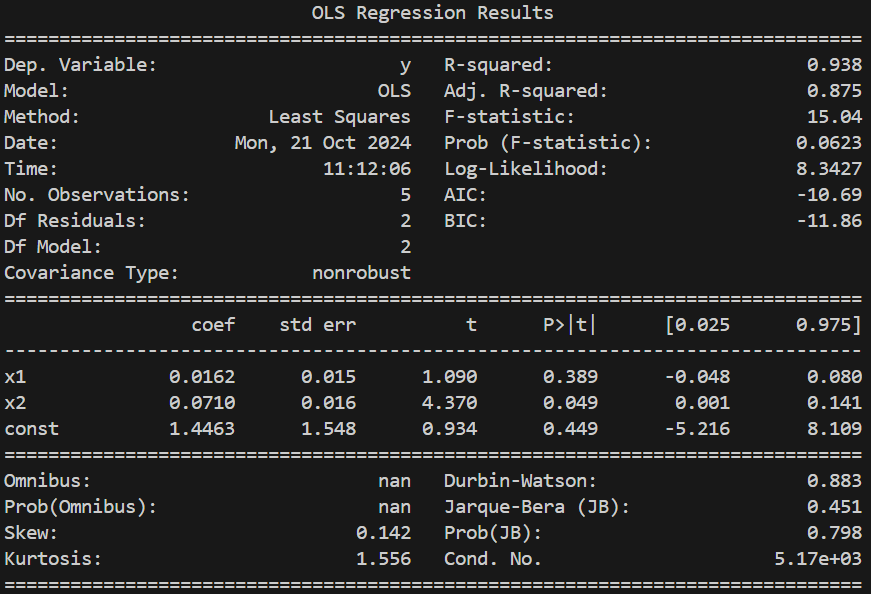
\includegraphics[width=\textwidth]{graphics/OLS_table.png}

\section{Exercise}

\begin{Exercise}
Show that if $A$ is an invertible $n \times n$ square matrix then the least-square solution of $A\vec{x} = \vec{h}$ given in Theorem \ref{thm:bestfit}
\begin{align*}
\vec{x}_f &= (A^\dag A)^{-1}A^\dag \vec{h}    
\end{align*}
will be reduced to simply
\begin{align*}
\vec{x}_f &= A^{-1}\vec{h}    
\end{align*}
the exact solution as derived in Section \ref{subsection:SolLinSysInv}.
\end{Exercise}

\begin{Exercise}
Find the least-square solution to the overdetermined linear system below.
\begin{align*}
\begin{cases}
x + 2y - 3z = 4 \\
x - y + 3z = 5 \\
2x + y - z = 1 \\
x + y + z = 2
\end{cases}
\end{align*}
\end{Exercise}

\begin{Exercise}
Find a linear fit for the following data about sea level pressure and temperature measured at a weather station.
\begin{center}
\begin{tabular}{|c|c|c|c|c|c|c|}
\hline
Temperature ($^\circ$ C) & 10 & 12 & 12 & 13 & 16 & 17\\
\hline
Pressure (hPa) & 1022.1 & 1019.5 & 1018.9 & 1017.6 & 1014.3 & 1013.5\\
\hline
\end{tabular}
\end{center}
\end{Exercise}

\begin{Exercise}
Find a linear fit and a quadratic fit for the following atmospheric data regarding global carbon dioxide level. Also, calculate the root-mean-square error for each fit.
\begin{center}
\fbox{
\includegraphics[scale = 0.3]{carbon.png}}
\end{center}
\begin{center}
\begin{tabular}{|c|c|c|c|c|c|c|}
\hline
Years passed since 1960 & 0 & 5 & 10 & 15 & 20 & 25 \\
\hline
CO$_2$ level (ppm) & 316.9 & 320.0 & 325.7 & 331.1 & 338.8 & 346.4 \\
\hline
Years passed since 1960 & 30 & 35 & 40 & 45 & 50 & 55\\
\hline
CO$_2$ level (ppm) & 354.4 & 361.0 & 369.7 & 380.0 & 390.1 & 401.0\\
\hline
\end{tabular}
\end{center}
(Data from: \href{https://gml.noaa.gov/webdata/ccgg/trends/co2/co2_mm_mlo.csv}{NOAA (https://gml.noaa.gov/webdata/ccgg/trends/co2/\\co2\_annmean\_mlo.csv)})
\end{Exercise}

\begin{Exercise}
Radioactive decay is modeled by $N = N_0e^{-kt}$, where $N_0$ and $k$ are the initial concentration and the decay constant respectively. While the formula is exponential, not linear, the technique of linear regression can still be applied if the data undergoes \textit{linearization}. Show that by the substitution $n = \ln N$ the equation can be transformed into a linear equation $n = \ln N = \ln N_0 - kt = n_0 - kt$. Hence find the best linear fit on $(t, n)$ by finding the parameters $(n_0, k)$ from the experimental data on the radioactive isotope Sodium-24 below and recover the decay constant and initial mass.
\begin{center}
\begin{tabular}{|c|c|c|c|c|c|c|}
\hline
Time passed (hr) & 6 & 8 & 12 & 24 & 36 & 48\\
\hline
Mass (g) & 75.8 & 69.1 & 57.3 & 33.0 & 18.8 & 10.8\\
\hline
\end{tabular}
\end{center}
\end{Exercise}

\begin{Exercise}
A commercial study investigates eight companies that sell the same type of products and are also similar in size. The following table summarizes their revenues, R\&D expenses, employee wages, and amounts of advertisement (the last three items are normalized scores).
\begin{center}
\begin{tabular}{|c|c|c|c|c|}
\hline
& Revenues & R\&D & Wages & Advertisement \\
\hline
Company 1 & 135\% & 2.5 & 1.7 & 0.8 \\
\hline
Company 2 & 128\% & 1.6 & 1.8 & 1.5 \\
\hline
Company 3 & 119\% & 1.8 & 0.5 & 2.4 \\
\hline
Company 4 & 121\% & 0.3 & 1.5 & 1.2 \\
\hline
Company 5 & 126\% & 1.9 & 1.6 & 1.3 \\
\hline
Company 6 & 112\% & 0.8 & 1.1 & 0.2 \\
\hline
Company 7 & 143\% & 2.2 & 2.4 & 1.1 \\
\hline
Company 8 & 135\% & 1.5 & 2.2 & 2.3 \\
\hline
\end{tabular}
\end{center}
Construct a linear regression model for the revenue against the three factors that follow. What is the $R^2$ of this regression?
\end{Exercise} 